\subsection{GDT básica y pasaje a modo protegido}

\begin{enumerate}

\item[a)] Completamos la GDT de la siguiente manera: El primer descriptor se completa con ceros, ya que este debe ser nulo siempre; las siguientes 7 entradas no se usan debido a que se consideran ocupadas; la octava y la novena entrada corresponden a un descriptor de código de nivel 0 y 3 respectivamente; las dos siguientes son descriptores de datos de nivel 0 y 3 respectivamente. Para un mejor entendimiento observar la figura "GDT".

Los descriptores de segmento de código llevan un 8 en su campo type (EXECUTE ONLY) mientras que los de datos llevan un 2 (READ/WRITE). Para lograr direccionar los primeros 500MB de memoria, establecemos el límite en {\tt 0x1F3FF} y la granularidad en 1.

\item[c)] Asignamos la entrada 12 de la GDT para el área de pantalla. Se establece la base en {\tt 0xB8000} y su límite en {\tt 0x1000}, el campo type se define como 2 (READ/WRITE) y el bit S en 1. Una vez hecho esto, movemos el selector de esta entrada al registro de segmento FS.

\item[d)] Utilizamos la funcion {\tt inic_video} para limpiar la pantalla e inicializarla como muestra la figura \ref{fig:pantalla}. Hacemos uso de la estructura que se encuentra en {\tt screen.h} para ir asignando los distintos caracteres y sus atributos (color de caracter y su color de fondo). Para esto usamos la dirección física del buffer de video {\tt 0xB8000}.

%\begin{figure}[h]
%	  \centering
%	    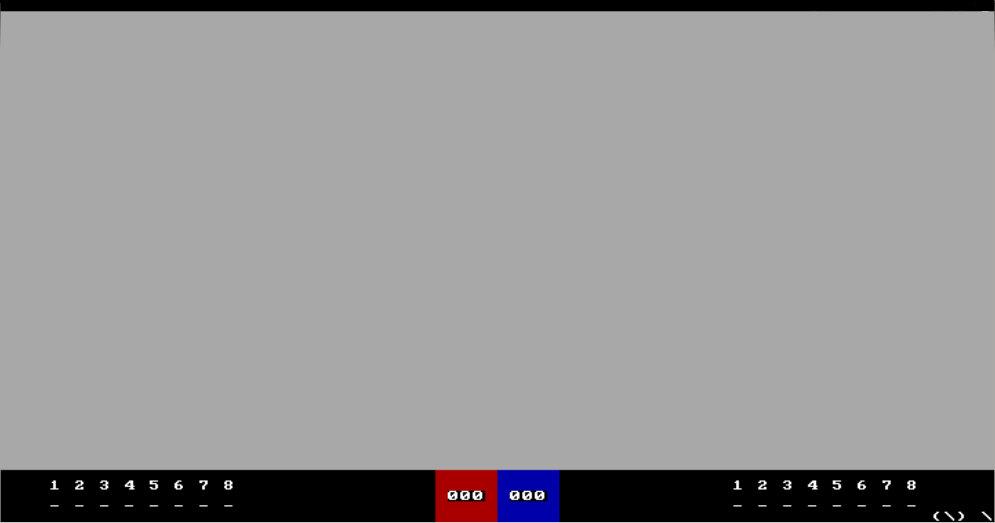
\includegraphics[ width=0.25\textwidth]{imagenes/pantallainicial.png}
%	     \caption{Pantalla inicializada}
%	  \label{fig:pantalla}
%	  \vspace{-15pt}
%	\end{figure}
%	\FloatBarrier
